\section{Thực nghiệm và thảo luận} % Section 3

\subsection{Kết quả phân tích}

\subsection{Biểu đồ , bảng biểu , hình ảnh minh hoạ}

\subsubsection{MobileNetV3Small}

\begin{table}[H]
\centering
\begin{tabular}{|l|l|}
\hline
\textbf{Tên kiến trúc} & \textbf{Độ chính xác (\%)} \\
\hline
MobileNetV3Small & 61.63 \\
MobileNetV3Small +  FER2013 LLI & 60.49 \\
MobileNetV3Small +  FER2013 LLI +  adaptive augmengution & 58.15 \\
\hline
\end{tabular}
\caption{Kết quả huấn luyện}
\end{table}
    
\begin{figure}[H]
\centering
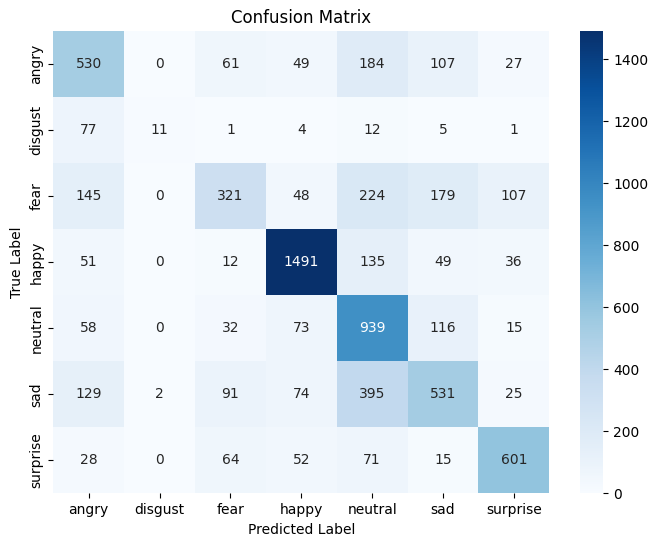
\includegraphics[width=1\textwidth]{img/confusionMatrixMobilenetV3.png}  % thay bằng tên file ảnh
\caption{Ma trận nhầm lẫn}
\end{figure}

\subsubsection{ResNet18}

\begin{table}[H]
\centering
\begin{tabular}{|l|l|}
\hline
\textbf{Tên kiến trúc} & \textbf{Độ chính xác (\%)} \\
\hline
ResNet18 & 67.23 \\
ResNet18 +  FER2013 LLI & 67.04 \\
ResNet18 +  FER2013 LLI +  adaptive augmengution & 67.48 \\
\hline
\end{tabular}
\caption{Kết quả huấn luyện}
\end{table}

\begin{figure}[H]
\centering
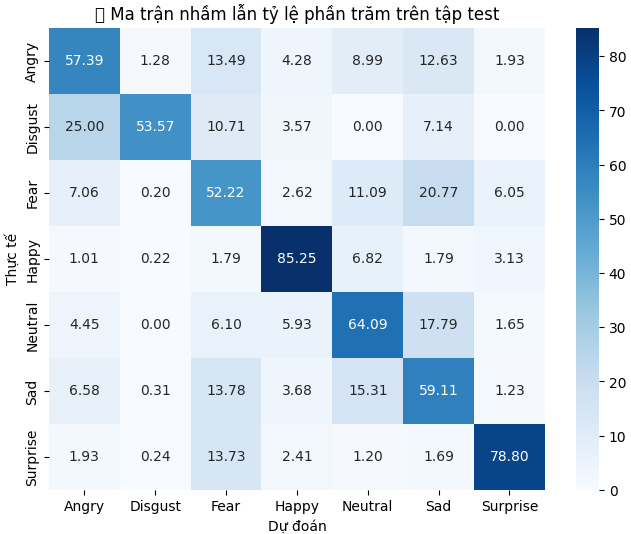
\includegraphics[width=1\textwidth]{img/confusionMatrixResnet18.png}  % thay bằng tên file ảnh
\caption{Ma trận nhầm lẫn}
\end{figure}
    
    

\subsection{Đánh giá  , giải thích kết quả nghiên  cứu}

\subsection{Nêu ý nghĩa thực tiễn của nghiên cứu}

\subsection{Những hạn chế , đề xuất nghiên cứu tiếp theo}